% Template: http://www.acm.org/sigs/publications/proceedings-templates#aL2 
% 
\documentclass{article}

\usepackage{amsmath}    % need for subequations
\usepackage{graphicx}   % need for figures
\usepackage{verbatim}   % useful for program listings
\usepackage{color}      % use if color is used in text
\usepackage{subfigure}  % use for side-by-side figures
\usepackage{hyperref}   % use for hypertext links, including those to external documents and URLs
\usepackage{url}
\usepackage{multicol}
\usepackage{textcomp}
%\usepackage{caption}  %% supported in class
\usepackage{algorithm}
\usepackage{algpseudocode}
\usepackage{enumitem}
\usepackage{mathtools}
\DeclarePairedDelimiter{\ceil}{\lceil}{\rceil}
%\usepackage{pstricks}
%\usepackage{authblk}  %% supported in class
% \usepackage{float}
% \newfloat{algorithm}{t}{lop}

\newcommand{\ndnrtcName}{NDN-RTC} % {\emph{ndnrtc}}
\newcommand{\ndnconName}{\emph{ndncon}}
\newcommand{\wConcept}{Interest demand}

\clubpenalty=10000 
\widowpenalty = 10000

%% Shrink lists - http://tex.stackexchange.com/questions/43743/how-to-reduce-line-space-leading-within-an-enumerate-environment 
\setenumerate{itemsep=-0.5ex,topsep=1ex, leftmargin=*}
\setitemize{itemsep=-0.5ex,topsep=1ex, leftmargin=*}

\title{NDN-RTC report}


\clubpenalty=10000 
\widowpenalty = 10000

%************************************************
\begin{document}

\maketitle

%************************************************
% \abstract


%************************************************
\section{\ndnrtcName{} Progress}

\ndnrtcName{} is a real-time videoconferencing application which provides functionality for establishing low-latency media (audio and video) streaming over NDN. \ndnconName{} is a GUI application that was built on top of \ndnrtcName{} in order to provide a replacement of audio-video conferencing tools for NDN community that leverages NDN Testbed. The project is aimed at wide adoption of \ndnconName{} for internal weekly meetings and seminars. 

A number of tests were performed since last year in order to improve and fine-tune algorithms for real-time data dissemination over NDN design during the first year of the project:
\begin{itemize}
\item \textbf{Latest data detection.} It is critical for consumer to reach the latest data available on the network in order to avoid unnecessarily increased delays. The previously introduced idea of \textbf{cache exhaustion} was re-formulated with focus on \textbf{getting the latest data}, which still may be cached. Consumers do not necessarily need to reach producer directly. In fact, in tests conducted, only one consumer in multi-consumer scenarios is reaching producers, while others receive cached data (\ref{fig:drd}). However, cached data does not mean old data. Consumers aim at getting ``latest" data from the network and implement techniques for detecting arrival of the latest data. These techniques are based on detecting stable values of inter-arrival delays of incoming packets which is the quality of the latest data. New approach of smoothing out inter-arrival delay values over two consecutive time windows gives much more robust results in detecting latest data.

\begin{figure}[t!]
\centering
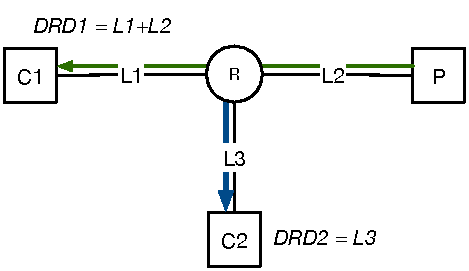
\includegraphics[width=0.45\textwidth]{drd}
\caption{Data Retrieval Delays in 1-to-2 RTSD fetching scenario:  $C2$ experiences smaller $DRD$ value when it starts fetching after the $C1$ and receives cached data from the  $R$.}
\label{fig:drd}
\end{figure}

\item \textbf{Controllable consumer aggressiveness.} A consumer maintains a pipeline of outstanding Interests for the future data and expresses more Interests when new Data arrives. New Interest ``bursting" and ``withholding" techniques allow consumer to tune expression pattern in order to react quickly for changing conditions, like buffer starvation or old data arrival.
\item \textbf{Performance improvements.} A number of implementation improvements were made affecting overall library performance and robustness: single-threaded consumers, asynchronous non-blocking logging, CPU load and memory footprint optimizations.
\end{itemize}

A new headless application was developed in order to facilitate experiments with NDN-RTC by other research groups. Headless application is cross-platform: OSX and Ubuntu are currently supported. It can be built from sources or downloaded as a part of NDN-RTC Docker image for easy and fast setup. Releasing this image was crucial for enabling research work on congestion control algorithms for NDN. Same image will be used in future large-scale tests, providing easiness in setup and results gathering.

\section{Findings}

Having operating application like \ndnconName{} allows to continuously check proposed congestion control algorithms and test them in real life immediately, thus delivering working solutions faster and incorporate ideas in working code to drive research further.

Generalizing NDN-RTC design (\ref{fig:consumer-producer}) allowed to adapt its' techniques to use in other NDN applications that require real-time data dissemination: live person tracking (OpenPTrack) and distributed control system for live performance (Ananke). Reviewing and generalization of conducted work helps for establishing new concepts ($DRD$ - Data Retrieval Delay instead of conventional RTT, \textit{Interest demand} - minimal amount of oustanding Interests required to establish real-time streaming) which describe NDN environment more accurately and help to evade dangerous TCP/IP analogies.

\begin{figure}[t!]
\centering
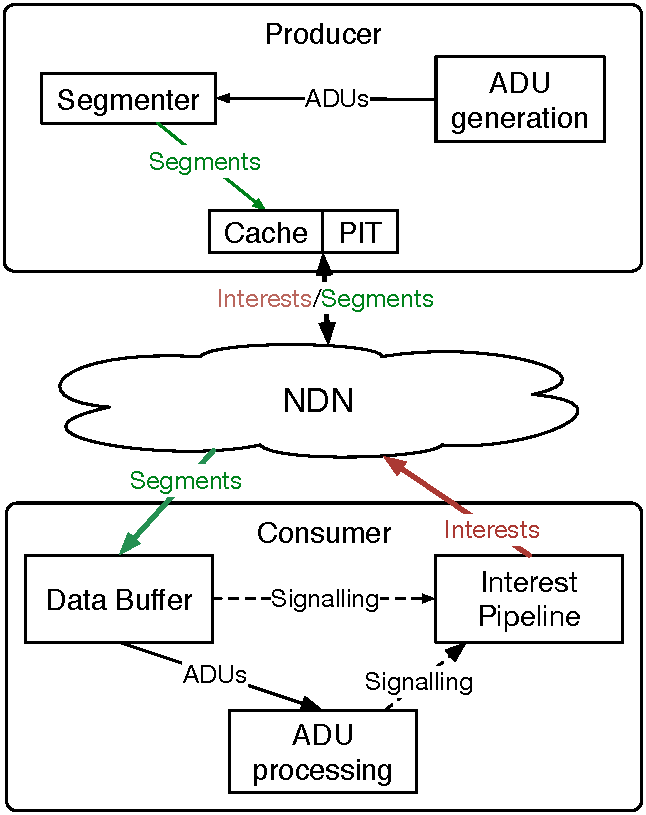
\includegraphics[width=0.3\textwidth]{consumer-producer-general}
\caption{NDN consumer and producer conceptual design.}
\label{fig:consumer-producer}
\end{figure}

Experience of using \ndnconName{} for seminars revealed the importance of running these kind of tests on ongoing basis for testbed consistency checking. A number of important issues were revealed, such as CPU and memory load of NFD, testbed strategy configurations on certain hubs, properly configured and functioning testbed prefix auto-registration and auto-propagation, legitimate users and guests certificate management.

\section{Public presentations}
\begin{enumerate}
\item Peter Gusev ``NDN-RTC project updates", NDN Community Meeting, Sept. 2015
\end{enumerate}

\section{Citations}
\begin{itemize}
\item \cite{ndnrtc}
\item \cite{ntsd}
\end{itemize}

\bibliographystyle{abbrv}
{\small
\bibliography{bibliography}
}


\end{document}